\documentclass[11pt,aspectratio=169]{beamer}
\usetheme{default}
\usecolortheme{seahorse}
\setbeamertemplate{navigation symbols}{}
\setbeamertemplate{footline}[frame number]
\usepackage{booktabs}
\usepackage{amsmath,amssymb}
\usepackage{tikz}
\usetikzlibrary{arrows.meta,positioning,fit,backgrounds}
\usepackage{xcolor}

\definecolor{trad}{HTML}{2e6fb7}
\definecolor{stab}{HTML}{c75b4a}
\definecolor{game}{HTML}{4d8b6f}
\definecolor{lo}{HTML}{f4f4f4}

\newcommand{\El}{\ensuremath{\Pi_{\text{risk}}}}

\title{The Risk-Adjusted Cost of Stablecoins as Payment Instruments}
\subtitle{Pricing the payment workflow, leg by leg}
\author{Andr\'es Alonso-Robisco}
\institute{IE University \,\textbar\, Banco de Espa\~na}
\date{\today}

\begin{document}

\begin{frame}\titlepage\end{frame}

% ---------------------------------------------------------------------------
\begin{frame}{The number everyone quotes, and the cost it omits}
A US--Mexico retail payment:
\begin{itemize}
  \item SWIFT correspondent banking: \(\approx 330\) basis points (World Bank RPW).
  \item USDT on Tron: \(\approx 37\) basis points per transfer.
\end{itemize}
\vspace{1em}
The ninefold gap is the case for stablecoins as a payment frontier. \\[0.6em]
\textbf{But the announced fee prices only the on-chain hop.} The sender holds a
private-issuer liability and runs a full \emph{fiat-to-fiat circuit}. We price
that circuit, leg by leg.
\end{frame}

% ---------------------------------------------------------------------------
\begin{frame}{The organising idea: compare two payment workflows}
\centering
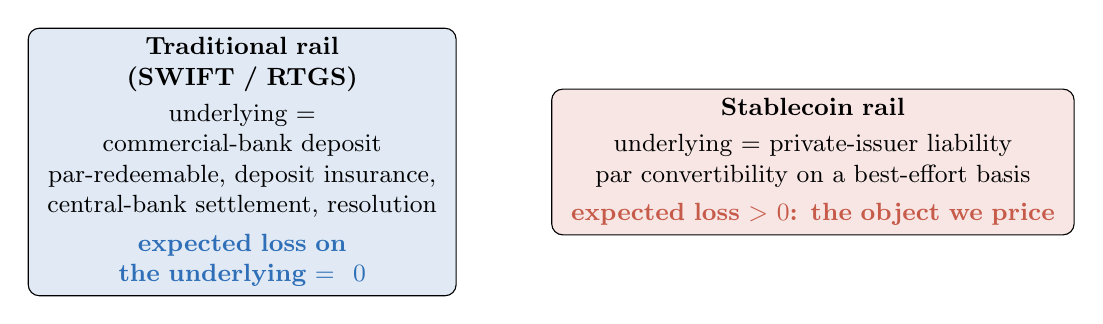
\begin{tikzpicture}[font=\small, >=Latex, node distance=4mm]
\node[draw, rounded corners, fill=trad!15, text width=5.2cm, align=center] (t) {%
  \textbf{Traditional rail (SWIFT / RTGS)}\\[2pt]
  underlying $=$ commercial-bank deposit\\
  par-redeemable, deposit insurance,\\
  central-bank settlement, resolution\\[3pt]
  \textcolor{trad}{\textbf{expected loss on the underlying $=0$}}};
\node[draw, rounded corners, fill=stab!15, text width=6.4cm, align=center, right=1.2cm of t] (s) {%
  \textbf{Stablecoin rail}\\[2pt]
  underlying $=$ private-issuer liability\\
  par convertibility on a best-effort basis\\[3pt]
  \textcolor{stab}{\textbf{expected loss $>0$: the object we price}}};
\end{tikzpicture}
\vspace{1em}
\begin{itemize}
  \item The rail's operational risk is common to both and nets out.
  \item What does \emph{not} net out is the asset the payer briefly holds.
  \item \(\El\) is the cost of replacing a publicly backstopped par promise with a private one.
\end{itemize}
\end{frame}

% ---------------------------------------------------------------------------
\begin{frame}{The traditional workflow: nothing to price on the underlying}
\centering
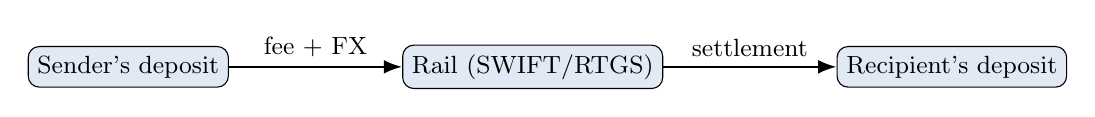
\begin{tikzpicture}[font=\small, >=Latex]
\node[draw, rounded corners, fill=trad!15] (a) {Sender's deposit};
\node[draw, rounded corners, fill=trad!15, right=2.2cm of a] (b) {Rail (SWIFT/RTGS)};
\node[draw, rounded corners, fill=trad!15, right=2.2cm of b] (c) {Recipient's deposit};
\draw[->, thick] (a) -- node[above]{fee + FX} (b);
\draw[->, thick] (b) -- node[above]{settlement} (c);
\end{tikzpicture}
\vspace{1.2em}
\begin{itemize}
  \item The payer holds a \textbf{par-redeemable claim} backstopped by deposit
        insurance, central-bank settlement, and orderly resolution.
  \item For a retail-sized payment: \textbf{no counterparty loss, no depeg loss}.
  \item The public backstops are exactly what prevents a system-level run, so
        there is nothing left to calibrate. \(\;\El^{\text{trad}} = 0.\)
\end{itemize}
\end{frame}

% ---------------------------------------------------------------------------
\begin{frame}{The stablecoin workflow: five legs, fiat to fiat}
\centering
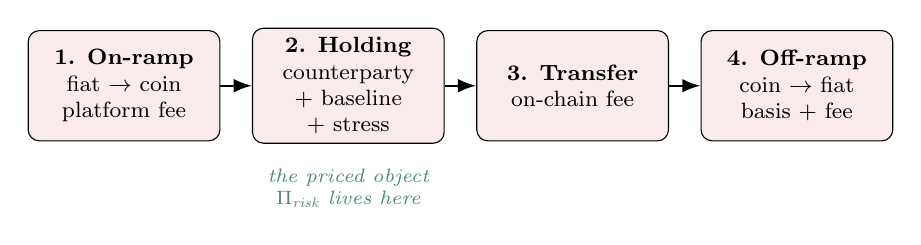
\begin{tikzpicture}[font=\footnotesize, >=Latex, node distance=3mm,
  leg/.style={draw, rounded corners, fill=stab!12, text width=2.2cm, align=center, minimum height=1.4cm}]
\node[leg] (on)  {\textbf{1. On-ramp}\\ fiat $\to$ coin\\ platform fee};
\node[leg, right=4mm of on] (hold) {\textbf{2. Holding}\\ counterparty\\ + baseline\\ + stress};
\node[leg, right=4mm of hold] (chain) {\textbf{3. Transfer}\\ on-chain fee};
\node[leg, right=4mm of chain] (off) {\textbf{4. Off-ramp}\\ coin $\to$ fiat\\ basis + fee};
\draw[->, thick] (on)--(hold); \draw[->, thick] (hold)--(chain); \draw[->, thick] (chain)--(off);
\node[below=2mm of hold, text width=3.2cm, align=center, font=\scriptsize\itshape, game] {the priced object \El\ lives here};
\end{tikzpicture}
\vspace{0.8em}
\begin{itemize}
  \item Legs 1, 3, 4 are \textbf{observable fees} (platform, gas, basis).
  \item Leg 2 is the \textbf{expected loss on the liability} the sender holds:
        counterparty $+$ depeg. That is where the model works.
\end{itemize}
\end{frame}

% ---------------------------------------------------------------------------
\begin{frame}{Leg 2a --- counterparty risk (observable, no model)}
The holder of one unit faces an annualised default hazard \(h\) and loss given
default \(\xi\). Over the working-balance horizon \(T=1\):
\[
  \ell_C = h\,\xi \times 10^4 \quad\text{basis points.}
\]
\textbf{Read from market proxies, not calibrated:}
\begin{itemize}
  \item \(\xi\): attested reserve composition (Circle daily disclosure vs Tether BDO attestations).
  \item \(h\): enforcement record (NYAG/CFTC) mapped to BB--B one-year default frequencies.
\end{itemize}
\vspace{0.5em}
\begin{center}
\begin{tabular}{lccc}
\toprule
 & \(h\) & \(\xi\) & \(\ell_C\) (bps) \\
\midrule
USDC & 0.01 & 0.20 & 20 \\
USDT & 0.02 & 0.30 & 60 \\
\bottomrule
\end{tabular}
\end{center}
\end{frame}

% ---------------------------------------------------------------------------
\begin{frame}{Leg 2b --- baseline depeg (approximated from the secondary)}
In normal times the par claim still costs something to convert: the realised
conversion price sits below par by the secondary-market spread.
\begin{itemize}
  \item At the USD-pair mid the below-par expectation is tiny (\(0.4\)--\(2\) bps over 38{,}688 hours).
  \item The holder does not exit at the mid: the off-ramp spread is an order of magnitude wider.
  \item We take the \textbf{observed off-ramp basis} as \(\ell_{D,b}\): \(\approx 21\) bps (BRL), \(12\) bps (MXN).
\end{itemize}
\vspace{0.5em}
\centering
\textcolor{game}{The linear coordination model has zero baseline mid-depeg by
construction \(\Rightarrow\) the baseline is an observable, not a model output.}
\end{frame}

% ---------------------------------------------------------------------------
\begin{frame}{Leg 2c --- stress depeg: a coordination run (the global game)}
When many holders convert at once, primary redemption is exhausted and the
secondary price falls --- a self-fulfilling run. Two episodes, opposite poles:
\begin{center}
\begin{tabular}{lcccc}
\toprule
Coin & Episode & Primary redemption & Trough & Mean depth \\
\midrule
USDC & SVB, Mar 2023   & constrained (bank weekend) & 0.902 & 240 bps \\
USDT & Terra, May 2022 & stayed open at par         & 0.975 & \phantom{0}28 bps \\
\bottomrule
\end{tabular}
\end{center}
\vspace{0.6em}
The depth of a depeg turns on \textbf{whether primary redemption survives the
shock} --- exactly the reserve channel the model formalises. This is the one
piece no observable conversion cost reveals.
\end{frame}

% ---------------------------------------------------------------------------
\begin{frame}{The global game, closed form (à la Klee)}
Uniform signal noise + linear price impact + dual-channel exit (primary up to
reserves \(R\), residual to a secondary with depth \(1/\psi\)):
\[
  \ell_D = \frac{\psi\,(-3AR + 3A - R^{3}\sigma + 3Rs^{*} - 3s^{*} + \sigma)}{3(A-B)},
  \qquad
  p_s = \frac{A + 2R\sigma - s^{*} - \sigma}{A - B}.
\]
\begin{itemize}
  \item Threshold \(s^{*}\): a \textbf{single one-dimensional} indifference equation (not a seven-parameter fit).
  \item \(\displaystyle \frac{\partial \ell_D}{\partial R} < 0\): deeper reserves lower the expected depeg loss --- \textbf{a theorem, not a simulation}.
  \item \(p_s\) is \textbf{endogenous and per coin} (Klee-style run probability), not a shared frequency.
\end{itemize}
\centering
\textcolor{game}{Causal/counterfactual properties are analytical; the level is contrasted with econometrics.}
\end{frame}

% ---------------------------------------------------------------------------
\begin{frame}{Leg 4 --- off-ramp, and the assembled expected loss}
Convert the coin back to local fiat: platform fee \(+\) destination basis.
\vspace{0.4em}
\begin{center}
\begin{tabular}{lccc}
\toprule
Expected-loss component & USDC & USDT & source \\
\midrule
\(\ell_C\) counterparty            & 20.0 & 60.0 & market proxies \\
\(\ell_{D,b}\) baseline depeg       & 26.4 & 10.9 & observed basis \\
\(\ell_{D,s}\) stress depeg (wtd)   & \phantom{0}2.6 & \phantom{0}0.3 & global game \(\times\,p_s\) \\
\midrule
\(\El\) total                       & \textbf{48.9} & \textbf{71.2} & \\
\bottomrule
\end{tabular}
\end{center}
\vspace{0.4em}
\textbf{Inverted compositions:} USDC depeg-dominant, USDT counterparty-dominant.
The same machinery, two issuers, two opposite risk profiles.
\end{frame}

% ---------------------------------------------------------------------------
\begin{frame}{Risk premium: three use cases, full circuit}
Full circuit \(=\) on-ramp \(+\) on-chain fee \(+\) \El\ \(+\) basis \(+\) off-ramp,
against public, incumbent, and fintech rails.
\begin{center}
\begin{tabular}{llrrl}
\toprule
Use case & Coin & Stablecoin (bps) & Best alternative & Outcome \\
\midrule
BR domestic \$40   & USDT & 517 & PIX (0)    & \textcolor{trad}{dominated} \\
US--MX \$400       & USDT & 171 & Wise (251) & \textcolor{stab}{wins by 80} \\
EU--BR \$1{,}000   & USDC & 135 & Wise (205) & \textcolor{stab}{wins by 70} \\
\bottomrule
\end{tabular}
\end{center}
\vspace{0.5em}
\begin{itemize}
  \item Dominated where an upgraded public rail already exists (PIX).
  \item Wins where none does, net of the full circuit.
  \item A projected BIS Nexus rail (5 / 2 bps) absorbs the advantage where it wins.
\end{itemize}
\end{frame}

% ---------------------------------------------------------------------------
\begin{frame}{Policy: one category, two instruments}
\begin{columns}
\begin{column}{0.5\textwidth}
\textbf{Heterogeneity}
\begin{itemize}
  \item USDC: depeg-dominant \(\Rightarrow\) supervise secondary-market depth and liquidity.
  \item USDT: counterparty-dominant \(\Rightarrow\) supervise reserve composition and attestation.
  \item A single rulebook misprices one of them.
\end{itemize}
\end{column}
\begin{column}{0.5\textwidth}
\textbf{Build vs license}
\begin{itemize}
  \item Where it wins, the stablecoin fills an infrastructure gap.
  \item An interlinked public instant-payment rail delivers the same settlement without the risk loading.
  \item \(\partial \El / \partial R < 0\): reserve and liquidity regulation reprice the premium directly.
\end{itemize}
\end{column}
\end{columns}
\end{frame}

% ---------------------------------------------------------------------------
\begin{frame}{Takeaways}
\begin{enumerate}
  \item The announced fee omits a structural expected loss on the liability the sender holds.
  \item We price it leg by leg: counterparty and baseline are \textbf{observable};
        the stress run is the \textbf{global game}, closed form, with an endogenous per-coin \(p_s\).
  \item USDC 49 bps (depeg-dominant) vs USDT 71 bps (counterparty-dominant): \textbf{two instruments, not one category}.
  \item Over the full circuit the stablecoin is dominated where a public rail exists,
        wins where none does, and is absorbed once an upgraded public cross-border rail goes live.
\end{enumerate}
\vfill
\centering\small The model earns its place through mechanism and counterfactuals; the number is disciplined by observables.
\end{frame}

\end{document}
